% ============================================================================
% CCA2 manuscript -- FIRST FULL DRAFT (2026-11-19)
%
% Target venue: Mathematical Programming Computation.
% NOTE: the MPC journal class (mpc.cls) is not available in this environment
% (checked: not installed locally, not on CTAN, not downloadable from the
% Springer pages), so this draft builds on the standard `article` class.
% Rebuild with the journal class at the revision stage.
%
% Ground rules for this draft (task requirement):
%  * Every number or repository-backed claim carries a "% CITE:" comment
%    naming the committed file, test or results file that supports it.
%  * Open gaps G3 (external comparison) and G5 (release tag + code DOI) are
%    marked  % TODO(G3) / % TODO(G5)  and are NOT claimed in the text.
%  * Prose is complete and correct but deliberately not polished; it will be
%    revised later.
%
% Build:   cd manuscript && ./build.sh     (or: latexmk -pdf main.tex)
% Biblio:  python3 ../biblio/tools/bibsubset.py main.tex   (see build.sh)
% ============================================================================
\documentclass[11pt]{article}

\usepackage[margin=2.6cm]{geometry}
\usepackage{amsmath,amssymb,amsthm}
\usepackage{booktabs}
\usepackage{natbib}
\usepackage{graphicx}
\usepackage{xcolor}
\usepackage{tikz}
\usepackage{pgffor}
\usepackage{enumitem}
\usepackage[hyphens]{url}
\usepackage{hyperref}
\hypersetup{colorlinks=true, linkcolor=blue!60!black, citecolor=blue!60!black,
            urlcolor=blue!60!black, pdftitle={Exact Conjugates and Convex Envelopes of
            Bivariate Piecewise Quadratic Functions}}

\newtheorem{theorem}{Theorem}
\newtheorem{lemma}[theorem]{Lemma}
\newtheorem{proposition}[theorem]{Proposition}
\newtheorem{corollary}[theorem]{Corollary}
\newtheorem{definition}[theorem]{Definition}
\theoremstyle{definition}
\newtheorem{remark}[theorem]{Remark}
\newtheorem{example}[theorem]{Example}

\newcommand{\R}{\mathbb{R}}
\newcommand{\Q}{\mathbb{Q}}
\newcommand{\E}{\mathbb{E}}
\DeclareMathOperator{\dom}{dom}
\DeclareMathOperator{\cl}{cl}
\DeclareMathOperator{\conv}{conv}
\DeclareMathOperator{\co}{co}
\DeclareMathOperator{\supp}{supp}
\DeclareMathOperator{\argmax}{argmax}
\DeclareMathOperator{\rank}{rank}
\DeclareMathOperator{\disc}{disc}

\title{Exact Conjugates and Convex Envelopes of Bivariate Piecewise Quadratic
       Functions: Algorithms, Proofs, and a Verified Implementation}

% TODO (drafting): verify affiliation and add co-authors at the revision stage.
\author{Yves Lucet\thanks{Department of Mathematics, University of British
        Columbia, Vancouver, Canada. \texttt{y.lucet@ubc.ca}.}}

\date{\today}

\begin{document}
\maketitle

\begin{abstract}
We compute the Fenchel conjugate and the biconjugate (closed convex envelope) of
nonconvex bivariate piecewise linear--quadratic (PLQ) functions \emph{exactly},
as closed-form piecewise objects with rational or algebraic data, without grid
sampling, LP relaxation or a computer algebra system in the compute path. Three
contributions. First, a direct exact-arithmetic algorithm for each operator,
whose output is one of three typed objects (piecewise quadratic, algebraic
curve, min-of-maxes) determined by the face type of the answer; the face types
themselves are new mathematical objects: face functions and edge conics of the
conjugate are always rational, its vertices have degree at most~$4$ (and degree~$4$
with Galois group~$S_4$ is attained), and the biconjugate carries algebraic
faces of degree~$4$ while failing to be $C^1$. A three-piece example refutes the
parabolic-subdivision claim of the published linear-time algorithms. Second, a
verification harness of four oracles that share no code with the engine it
checks -- golden replay, a pointwise definition oracle, a symbolic kernel oracle,
and three-engine field-for-field parity -- against which every claim in this
paper is pinned by a committed test. Third, MATLAB, Python and Rust
implementations at parity on a 200-fixture corpus, with the Rust engine
parallelised; on that corpus the best engine is roughly two orders of magnitude
faster than the symbolic MATLAB reference (indicative timings on a shared
machine). The paper states, with the same care, what is not yet established:
a small class of inputs on which the biconjugate is still slightly low, the
absence of an independent external comparison, and the absence of a citable
release.
\end{abstract}

% ============================================================================
\section{Introduction}
% ============================================================================

A bivariate piecewise linear--quadratic (PLQ) function is a function
$f:\R^2\to\R\cup\{+\infty\}$ that equals one of finitely many quadratic
polynomials on each cell of a polyhedral subdivision of $\R^2$; we assume
continuity on the domain (the case our algorithms are built for) and allow
nonconvex pieces and unbounded cells. Two operators on such functions are the
subject of this paper. The \emph{Fenchel conjugate}
\[
  f^*(s) \;=\; \sup_{x\in\dom f}\bigl(\langle s,x\rangle - f(x)\bigr),
\qquad s\in\R^2,
\]
and the \emph{biconjugate} $f^{**} = (\co f)^*$, the closed convex envelope of
$f$ (the largest closed convex minorant).
% CITE: definition standard,
% ROCKAFELLAR-70a in the bibliography; the operator list in README.md
 Both
operators are convex even when $f$ is not, which is exactly what makes them
useful: the conjugate of a nonconvex PLQ function is a convex PLQ-like object,
and the convex envelope is the strongest convex relaxation one can attach to a
nonconvex term.

\paragraph{Why exact closed form.}
Convex envelopes of nonconvex bilinear and quadratic terms are the workhorse of
global optimization: on the box-domain bilinear terms of the QPLIB benchmark
family, the envelope is the McCormick envelope, i.e.\ the Al-Khayyal--Falk
closed form~\cite{MCCORMICK-76,ALKHYAYAL-83}. This paper's toolbox reproduces
that closed form as a special case and is pinned to it by the test
\texttt{biconjugateTest/bilinearOverABoxGivesTheMcCormickEnvelope}.
% CITE: MATLAB/biconjugateTest.m line 96; the reading in SCIP\_READINESS.md
% section~0
 Its interest is the part that closed form does not cover: domains
that are not boxes, and diagonal terms such as $x^2-y^2$ over a box, which the
box formulas do not reach.
% CITE: SCIP\_READINESS.md section 0, ``the finding that shapes the whole
% plan''
 The intended consumer is the SCIP global
solver~\cite{ACHTERBERG-09}, whose nonconvex quadratics are exactly sums of
terms of this kind.
% CITE: SCIP\_READINESS.md sections 0 and 0.0.1

For this exact problem, linear-time algorithms have been
published~\cite{KARMARKAR-25,KARMARKAR-25a}. Their implementations, however,
run on a symbolic computer algebra system, and their heaviest cases take more
than four hours.
% CITE: TODO.md ``Open now'', item 4: biconjCPLQ on the poly2
% kinks runs > 4 h
 The MATLAB reference implementation in the repository is
far from the compiled ports on those same fixtures.
% CITE: python/bench/RESULTS.md: 412--566 s per single slow fixture in MATLAB
% versus 5.4--7.6 s in Rust, see also rust/bench/RESULTS.md
 The exact engine
described in this paper exists to remove symbolic computation from the compute
path entirely, and to do the two computations -- conjugate and convex envelope
-- directly rather than as a detour.

\paragraph{The answer is richer than the published theory says.}
The published algorithms~\cite{KARMARKAR-25,KARMARKAR-25a} state that the
conjugate of a PLQ function is piecewise quadratic \emph{on a parabolic
subdivision} (their edge curves satisfy $b^2-4ac=0$). We show in Section~3
that this is false in general: a continuous three-piece example on one triangle
carries an elliptic edge of the conjugate's subdivision, and a
% CITE: doc/QuaConExample.md, ``Answer in one line'' and section 2
five-piece continuous example carries a vertex of the conjugate whose
coordinates have degree~$4$ over $\Q$ with Galois group $S_4$, so no tower of
square roots suffices.
% CITE: DECISIONS.md entry 2026-08-20; CONJ\_FIELD\_PROOF.md
% sections 4--5
 An exact implementation therefore needs a data structure that no
grid method expresses: rational face functions, rational edge conics, algebraic
vertices of degree at most~$4$, and implicit algebraic faces on the envelope
side. Section~3 states the bounds that make that structure finite; Sections~4
and 5 describe the machinery that fills it.

\paragraph{Contributions.}
Three, in the order of the paper.
\begin{enumerate}[label=(\roman*), leftmargin=*]
\item \textbf{New exact algorithms} for the conjugate and the biconjugate of
  bivariate PLQ functions, in exact arithmetic, returning typed closed-form
  objects (Section~4 for the conjugate, Section~5 for the biconjugate). The
  mathematics behind the algorithm -- the face-type bounds of Section~3 --
  includes the three-piece refutation of the parabolic-subdivision claim of
  \citet{KARMARKAR-25} and the degree-$4$/$S_4$ vertex.
\item \textbf{A verification harness that owes nothing to the engine it
  checks}: a golden replay corpus, a pointwise definition oracle, a symbolic
  kernel oracle, and three-engine parity (Section~6). The harness is what makes
  the correctness claims of (i) checkable, and it is the reason a wrong value in
  the engine -- the star-polygon defect of Section~4 -- was found, localised to
  one routine, and fixed in all three languages.
  % CITE: DECISIONS.md entry 2026-11-17
\item \textbf{Three implementations at parity} -- MATLAB, Python, Rust -- with
  the Rust engine parallelised, and a reproducible 200-fixture benchmark
  protocol (Section~7). On that corpus the Rust engine is roughly two orders of
  magnitude faster than the MATLAB reference; we quote the numbers with their
  shared-machine caveats, not as a ranking (Section~7.4).
\end{enumerate}

The paper is a first full draft: the claims are complete, every one is tied to
a committed test, script or results file, and the open gaps -- one small
class of inputs on which the biconjugate is still slightly low (Section~8.5),
no independent external comparison
% TODO(G3): comparison against an independent external implementation or
% against grid/LP-based envelopes is missing from the repository (outline gap
% G3). The convexdb ground-truth registry that was to serve as the external
% oracle set has no Zenodo DOI yet. This is a gap, not a claim: do not add
% comparative numbers to Section 7 before it is closed.
and no citable release
% TODO(G5): no tagged release and no code DOI exist yet (outline gap G5;
% README.md ``Status'': alpha, API still changing). MPC wants a code archive
% with a DOI for the submitted version. Section 9 states this as a declared
% limitation; add the archive and DOI here at the revision stage.
-- are stated as such in Sections~8.5 and 9.

% ============================================================================
\section{The problem and prior work}
% ============================================================================

\subsection{Definitions and notation}

A \emph{quadratic} on $\R^2$ is a function
$q(x) = \tfrac12 x'Hx + \beta'x + \gamma$ with $H\in\R^{2\times2}$ symmetric,
$\beta\in\R^2$, $\gamma\in\R$. A bivariate PLQ function $f$ is given by a
polygon (possibly unbounded) subdivision $\mathcal T = (T_k)$ and a quadratic
$q_k$ on each cell $T_k$, with $f$ continuous on $\dom f$. The input type of
our algorithms, \texttt{QuaPol}, stores the vertices, edges, and the
$\{H_k,\beta_k,\gamma_k\}$, all with exact (rational) data.

The Fenchel conjugate $f^*$ is as in the introduction; the biconjugate
$f^{**}$ is $f^{**}(x) = \sup_s (\langle x,s\rangle - f^*(s))$, which for a
proper function equals $\cl\,\co f$ (the closed convex envelope).
% CITE: standard; ROCKAFELLAR-70a; the operator definitions in README.md and
% DESIGN.md
 We write $\langle s,x\rangle = s_1x_1+s_2x_2$.

Two conventions of the published papers, which we follow, matter for
Section~3. A \emph{parabolic} edge is a conic $ax_1^2+bx_1x_2+cx_2^2+\cdots=0$
with $b^2-4ac=0$; \citet{KARMARKAR-25,KARMARKAR-25a} call a function
\emph{piecewise parabolic} when its subdivision's edges are parabolas. A
\emph{rational function} in their sense is a quadratic divided by a linear
function. Both terms are defined on p.\,6 of \citet{KARMARKAR-25}.
% CITE: doc/QuaConExample.md section 1 quotes both definitions from the papers

\subsection{Prior work}

The two nearest predecessors are the linear-time algorithms of
\citet{KARMARKAR-25} (the conjugate, J.~Glob.\ Optim.) and
\citet{KARMARKAR-25a} (the convex envelope, Comput.\ Optim.\ Appl.). Both
handle nonconvex PLQ, both run in linear time for triangulated subdivisions,
and both are implemented in the repository as the legacy \texttt{'cplq'}
engine, which runs on the Symbolic Math Toolbox.
% CITE: README.md ``Algorithms and references''; the lineage and the mapping of
% each convex-only predecessor to the engine it would supply is in DESIGN.md
% ``PART I''
 Before them, the convex-only line: the
$\varepsilon$-subdifferential computation in worst-case optimal
time~\cite{KUMAR-18}, the biconjugate front-end for bivariate PLQ
~\cite{KUMAR-19,KUMAR-19a}, and the CCA toolbox for the convex operators.
% CITE: DESIGN.md lineage section; LUCET-CCA in the bibliography

Our starting point is the claim of \citet{KARMARKAR-25} that the conjugate of
a (nonconvex) PLQ function is piecewise quadratic on a \emph{parabolic}
subdivision (Theorem~6 and Proposition~7 of that paper). Section~3 shows the
claim is false in general, and the repository carries the counterexample
computed in full, exact rational arithmetic, with the proof of why the proof
breaks.
% CITE: doc/QuaConExample.md and doc/QuaConExampleProof.md
 This does
not invalidate the algorithms as computations on inputs where the claim holds;
it changes what an exact implementation must represent, and that is the
substance of Section~3.

\subsection{Scope}

The design target of the repository -- and of this paper -- is the conjugate
and biconjugate of a \texttt{QuaPol}: the two operators, for any bivariate PLQ
input with rational data, convex or not, bounded or not.
% CITE: CLAUDE.md ``What it is''; README.md operators table
 Cases that can
never arise from a \texttt{QuaPol} conjugate are \emph{out of scope by design,
not gaps}; the repository's support matrix records every guard as OK / GAP /
not-reachable / internal-invariant so that ``bug or by design'' is answerable
mechanically.
% CITE: SUPPORT\_MATRIX.md header and section 0 legend
The legacy \texttt{'cplq'} engine remains in the tree as the implementation of
\citet{KARMARKAR-25,KARMARKAR-25a} and as a cross-check; it is not the subject
of the correctness claims of this paper, and its open items are disclosed in
Section~9.2.

% ============================================================================
\section{What the answer looks like: face types and number fields}
% ============================================================================

This section states, with the bounds that make them finite, what the two
operators return on rational data. The full proofs are in the repository.
% CITE: CONJ\_FIELD\_PROOF.md (the conjugate side), DECISIONS.md entries
% 2026-08-20 and 2026-08-23 (the $S_4$ vertex and the envelope side),
% doc/QuaConExample.md (the counterexample)
 We restate the results and quote
the instances that attain the bounds.

\subsection{The conjugate: rational faces, rational edges, degree-$\le 4$ vertices}

Fix one piece $q+\iota_{T}$ and write
$g(s) = \sup_{x\in T}(\langle s,x\rangle - q(x))$. Where the supremum is
finite it is attained, and the maximiser is one of three
things.
% CITE: CONJ\_FIELD\_PROOF.md Lemma 1

\begin{lemma}[candidate value functions are rational quadratics]\label{lem:candidate}
Let $T$ be a rational polygon and $q$ a rational quadratic. For each cell of the
maximiser, the value function $g$ is one of:
\begin{itemize}[nosep,leftmargin=*]
\item a vertex $v$ of $T$: $g_v(s)=\langle s,v\rangle-q(v)$, a rational
  \emph{affine} function;
\item the relative interior of an edge: a rational quadratic of
  \emph{rank one};
\item an interior critical point (when $q$ is invertible): a rational quadratic
  of full rank,
  $g_{\mathrm{int}}(s)=\tfrac12(s-\beta)'Q^{-1}(s-\beta)-\gamma$.
\end{itemize}
All coefficients are rational.
\end{lemma}

\begin{theorem}[face type of $f^*$]\label{thm:conjface}
For a continuous PLQ $f$ with rational data:
\begin{itemize}[nosep,leftmargin=*]
\item every \emph{face function} of $f^*$ is one of the rational quadratics of
  Lemma~\ref{lem:candidate};
\item every \emph{edge curve} of the subdivision of $\dom f^*$ is a conic with
  rational coefficients (it lies in $\{A=B\}$ for two of them);
\item every \emph{vertex} of that subdivision is a point where at least three
  of the rational quadratics agree.
\end{itemize}
\end{theorem}

The proof is one sentence: $f^* = \max_k (q_k+\iota_{T_k})^*$, and a maximum
\emph{selects} among the functions of Lemma~\ref{lem:candidate}; it never
manufactures a new one.
% CITE: CONJ\_FIELD\_PROOF.md Theorem 1

\begin{theorem}[vertex degree]\label{thm:deg4}
Every vertex of the subdivision of $\dom f^*$ has coordinates algebraic of
degree at most~$4$ over $\Q$.
\end{theorem}

At a vertex three rational quadratics agree, so the vertex is a base point of
the pencil of two rational conics; two conics meet in at most four points, and
if they share a component the vertex lies on a rational line and the degree
drops to at most~$2$.
% CITE: CONJ\_FIELD\_PROOF.md Theorem 2
 The bound is
sharp, and the sharp case is as bad as algebra allows:

\begin{example}[$S_4$ vertex, five pieces, all convex]\label{ex:s4}
Take the triangle $\operatorname{conv}\{(24,10),(-16,10),(4,-20)\}$ fanned
from the interior point $(4,0)$ into three sub-triangles, each carrying a
positive-definite rational quadratic (so every piece is convex and every piece's
conjugate is its interior-critical branch). The three value functions
\[
\begin{aligned}
g_1(s)&= 2s_1^2+s_1s_2+\tfrac12 s_2^2+4s_1-2s_2, &
g_2(s)&= 2s_1^2+\tfrac12 s_2^2+2s_1+2s_2,\\
g_3(s)&= \tfrac12 s_1^2-s_1s_2+s_2^2-s_2+3
\end{aligned}
\]
meet at a genuine vertex $p\approx(0.6081,0.3585)$ of $f^*$ where all three
argmax points are strictly inside their triangles.
% CITE: DECISIONS.md entry 2026-08-20, ``Recomputed here''
 Eliminating $s_2$
from $g_1-g_2$ and $g_1-g_3$ gives the quartic
$3t^4-24t^3+10t^2+160t-96=0$, which is irreducible over $\Q$, has irreducible
resolvent cubic, and discriminant $32\,853\,221\,376$ (a non-square); those are
the standard certificates that its Galois group is $S_4$, of order~$24$.
% CITE: DECISIONS.md 2026-08-20, ``And it is a genuine vertex, not an
% artefact''; the independent re-check is .claude/s4VertexCheck.m
 Since $24$
is not a power of two, the point lies in \emph{no} iterated quadratic extension
of $\Q$.
\end{example}

So the vertices of $f^*$ are algebraic of degree at most~$4$, and the degree-$4$
case with full symmetric Galois group is attained on a fully convex input. This
is the part of the answer that no grid or square-root data structure can hold.

\subsection{The biconjugate: algebraic faces, and not $C^1$}

The envelope side is one conjugation further, and the face type degrades:

\begin{theorem}[face type of $f^{**}$]\label{thm:biconjface}
A face of $f^{**}$ coming from a ruled cell of the dual subdivision is
\emph{algebraic of degree at most~$4$}, generically of degree $4$ or $1$
(degree $2$ is possible only from adjacent primal pieces); in implicit form
$\Psi(x_1,x_2,z)=0$ it has degree~$4$ in $z$ and total degree at most~$8$.
Moreover $f^{**}$ is in general \emph{not} $C^1$: the gradient does not extend
across the images of the rank-deficient dual faces.
\end{theorem}

The mechanism:
% CITE: DECISIONS.md entry 2026-08-23, in full
on a ruled cell,
$f^{**}(x)=\langle s,x\rangle-f^*(s)$ with $s$ solving two conics -- the fixed
rational arc $g_i-g_j=0$ and the incidence conic whose coefficients are affine
in $x$ -- so the degree divides~$4$; and the degree-$2$ instance is explicit:
for
\[
 f = \begin{cases} x^2-y^2 & \text{on } [-1,1]\times[0,3],\\
                   x^2+y^2 & \text{on } [-4,4]\times[-3,0],\end{cases}
\]
continuous on the shared edge, the ruled cell carries
$f^{**}(x)=2x_1+6x_2-28+6\sqrt2\,\sqrt{(x_1-1)^2+(x_2-3)^2}$, whose implicit
form $(z-2x_1-6x_2+28)^2-72[(x_1-1)^2+(x_2-3)^2]=0$ is irreducible of
degree~$2$ in $z$.
% CITE: DECISIONS.md 2026-08-23, ``Degree 2 IS reachable''
The failure of $C^1$ is witnessed by $|x_1|+x_2^2$, a legal convex input whose
dual has one rank-$1$ face whose gradient image is a line.
% CITE: DECISIONS.md 2026-08-23, ``$f^{**}$ is NOT $C^1$''

The stored form is the \emph{parametrisation}, not the implicit polynomial:
with $H(\lambda)=(1-\lambda)H_i+\lambda H_j$ and likewise for $a,c$,
\[
 x(s,\lambda)=\operatorname{grad} g_\lambda(s),\qquad
 z(s,\lambda)=\langle s,x\rangle-f^*(s)=\tfrac12 s'H(\lambda)s-c(\lambda),
\]
which sweeps the face without root-finding.
% CITE: DECISIONS.md 2026-08-23,
% ``The parametrisation, which is what should be stored''
 This is the data
structure of the \texttt{AlgCrv} output type of Section~5.

\subsection{The counterexample to the parabolic-subdivision claim}

\begin{theorem}[$f^*$ need not be parabolic]\label{thm:counter}
There is a continuous PLQ function on a triangle, with three positive-definite
rational pieces, whose conjugate's subdivision carries a non-degenerate
\emph{elliptic} edge.
\end{theorem}

Take the triangle $\operatorname{conv}\{(0,0),(60,10),(-5,10)\}$ cut by the
two cevians to $(15,10)$ and $(5,10)$, with positive-definite rational
quadratics on the three pieces (data in the repository). On the horizontal
segment from $(\tfrac92,\tfrac32)$ to $(\tfrac72,\tfrac32)$ the maximiser of
$f^*$ switches from piece~1 to piece~3 \emph{across} the conic
\[
 93s_1^2+38s_1s_2-6s_1+39s_2^2-482s_2-1003=0,
\]
whose discriminant is $b^2-4ac=-13\,064<0$: an ellipse, and the $3\times3$
determinant $-8\,650\,208\ne0$ rules out a degenerate conic.
% CITE: doc/QuaConExample.md section 2, with the tie table
 The switching
point is $s^*=\bigl(\frac{-17}{62}+\frac{\sqrt{612\,030}}{186},\;\frac32\bigr)$,
where pieces 1 and 3 tie at $2.9278190688\ldots$ with piece 2 strictly below; a
brute-force sup of $\langle s^*,x\rangle-f(x)$ over about eight million sampled
points returns $2.92778$, a lower bound agreeing to five digits.
% CITE: doc/QuaConExample.md section 2, last paragraph

The break in the published proof is one sentence: it assumes the two functions
compared in the cross-piece maximum include a linear one, \emph{because the
pieces compared are adjacent}; with three or more pieces a compared pair is
non-adjacent and both functions can be elliptic quadratics, their difference a
general conic. The adjacent case remains true -- there the difference factors
through the shared edge into a pair of lines, which are legal parabolas.
% CITE: doc/QuaConExample.md section 1, ``Where the proof breaks'', and the
% re-check of the adjacent case on six random exact continuous pairs

\begin{example}[the five-piece instance, displayed]\label{ex:5piece}
The five-piece example of Section~3.1 in the repository conjugates to
$35$ cells, which merge to $23$ distinct formulas and then to
$\mathbf{17}$ faces; of its $41$ genuine edges, $31$ are straight (of which $8$
are pairs of lines, the adjacent-piece case), $5$ are elliptic arcs and $5$
hyperbolic arcs, and \emph{zero} are genuine parabolas.
% CITE: doc/QuaConExample.md section 3, ``The 17 faces'' and ``The edges''.
% The figure is Figure~\ref{fig:facemap}.
 The $S_4$ vertex of
Example~\ref{ex:s4} is one of its vertices: the point
$p\approx(3.9078,1.4146)$ where faces $I_1$, $I_3$, $I_5$ meet and nothing
else does.
% CITE: doc/QuaConExample.md section 3.2, face-map caption
\end{example}

\begin{figure}[t]
\centering
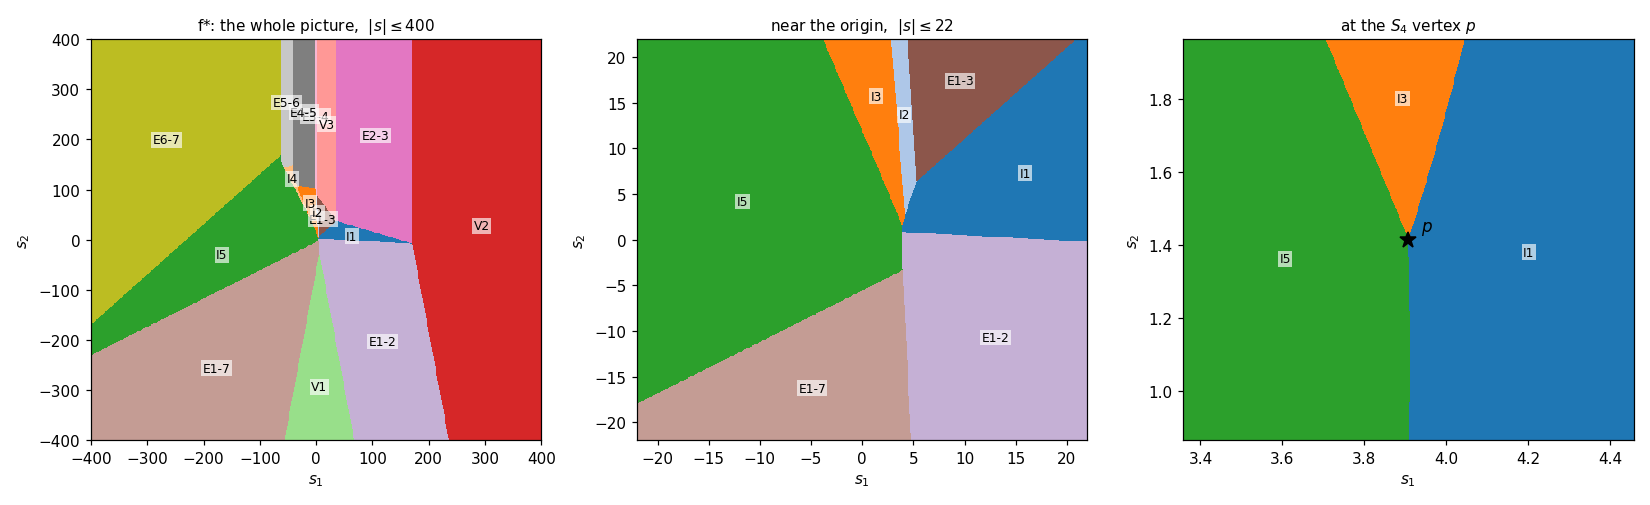
\includegraphics[width=\textwidth]{figures/QuaConExample-facemap.png}
\caption{The five-piece example of Example~\ref{ex:5piece}: which face of
$f^*$ attains the maximum, the whole arrangement, the crowded region near the
origin, and the $S_4$ vertex where $I_1$, $I_3$ and $I_5$ meet. Source:
\texttt{doc/QuaConExample-facemap.png}, computed by the MATLAB reference from
the data of \texttt{doc/QuaConExample.md}.}
\label{fig:facemap}
\end{figure}

\subsection{Consequence for the data structure}

The two theorems together fix the finite data structure an exact engine needs:
\emph{rational} face functions and edge conics on the conjugate side (Theorem
\ref{thm:conjface}), \emph{algebraic} vertices of degree at most~$4$
(Theorem~\ref{thm:deg4}), and \emph{algebraic} faces of degree at most~$4$ on
the envelope side (Theorem~\ref{thm:biconjface}). A grid method cannot express
any of the last two; a tower-of-square-roots type cannot hold
Example~\ref{ex:s4}. The output types of the engine -- \texttt{QuaCon},
\texttt{AlgCrv}, \texttt{EnvelopeMin} (Section~5) -- are exactly this
structure, and the refusal identifiers of Section~5 are exactly its boundary.

% ============================================================================
\section{The exact conjugate}
% ============================================================================

\subsection{The order of operations}

The conjugate of a PLQ function is, cell by cell, a small number of closed
forms; the difficulty is assembly -- taking the maximum across cells and
across pieces -- and the assembly is where a symbolic detour, or a triangulation
that was not needed, costs minutes or hours. The repository's design principle
is \emph{classify first, split last, and prefer the direct operator}: the same
mathematics costs seconds or hours depending on when each question is asked.
% CITE: ALGORITHM.md, ``The governing principle''; the measured cost of getting
% the order wrong is there too -- $(x^2+y^2)/2$ over the unit square cost $456$~s
% through the split-and-reassemble route against $4.2$~s through the direct
% route, and $x^2-y^2$ went from an error to an exact answer in $1.9$~s by
% testing separability before the change of variables
% [CITE: ALGORITHM.md, ``Measured effect of getting the order right'']

Concretely, for \texttt{conj($f$)}:
\begin{enumerate}[leftmargin=*]
\item \textbf{Normalise.} Merge adjacent faces carrying the same quadratic
  (exact equality of coefficients, not to $10^{-12}$); a merge is admitted only
  if its union is convex, checked with the subdivision's own convexity test.
  % CITE: ALGORITHM.md, Step 0 discussion, with the measured fan counterexample
\item \textbf{Separable on a box:} conjugate each axis in one dimension and
  add; this is tested \emph{before} any change of variables, because an
  indefinite diagonal quadratic such as $x^2-y^2$ is separable as written and
  rotating it into the $xy$ frame destroys the box.
  % CITE: ALGORITHM.md, ``Why the triangulation exists''
\item \textbf{Per piece, classify by the sign of the Hessian} (free: the
  $2\times2$ \texttt{eig}):
  \begin{itemize}[nosep,leftmargin=*]
  \item \emph{convex/affine}: the envelope is $f$ itself; the cells are the
    KKT active sets -- one per vertex, one per edge, one interior -- on the
    polygon as it stands, with no triangulation.
    % CITE: ALGORITHM.md, conjugate dispatch, convex bullet
  \item \emph{concave}: the envelope is the affine interpolant of the vertex
    values over the lower hull; the conjugate is the support function.
    % CITE: ALGORITHM.md, concave bullet
  \item \emph{indefinite}: change variables to the $xy$ frame, triangulate, and
    apply the closed forms of \citet{KARMARKAR-25} classified by convex-edge
    count (A.2--A.5, with the A.5 split when three edges are convex); the
    split point is a \emph{determined} point and must not be moved -- moving it
    turns the closed form into a strict minorant, which is exactly the defect
    the old A.4 branch carried.
    % CITE: ALGORITHM.md, indefinite bullet and ``Rational split points''
  \end{itemize}
\item \textbf{Maximum across pieces, last,} and only if more than one piece
  survived.
  % CITE: ALGORITHM.md, conj dispatch Step 3
\end{enumerate}

Every decision in the assembly -- which face is live on a cell, which rows drop,
whether a cell has an interior -- is the sign of a rational number computed in
exact arithmetic; doubles appear only for sampling and for the polynomial
kernels that have a symbolic oracle (Section~6.1).
% CITE: TODO.md 2026-09-06 entry, ``the exact evaluator''; DECISIONS.md entry
% 2026-08-19, ``the symbolic-removal list''; python/bench/RESULTS.md ``What ran''

\begin{figure}[t]
\centering
\begin{minipage}[b]{0.48\textwidth}\centering
  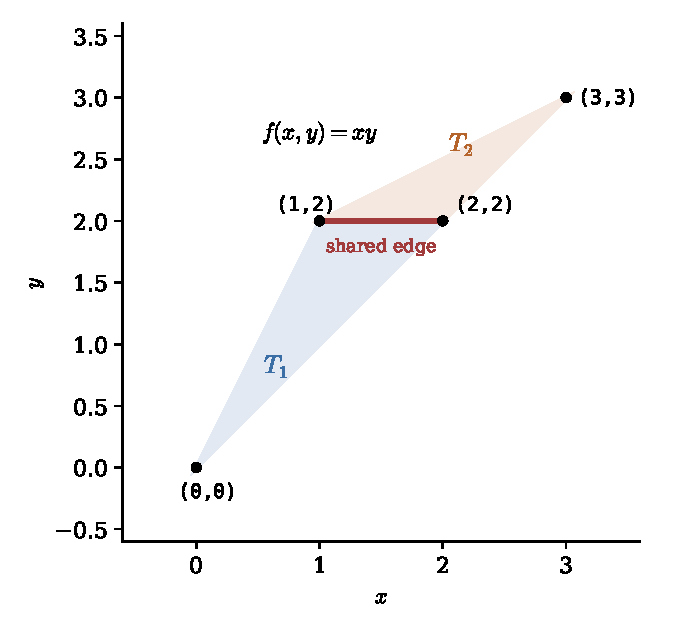
\includegraphics[width=\linewidth]{figures/fig_primal.pdf}\\
  \small the primal: $f=xy$ on a two-cell quadrilateral
\end{minipage}\hfill
\begin{minipage}[b]{0.48\textwidth}\centering
  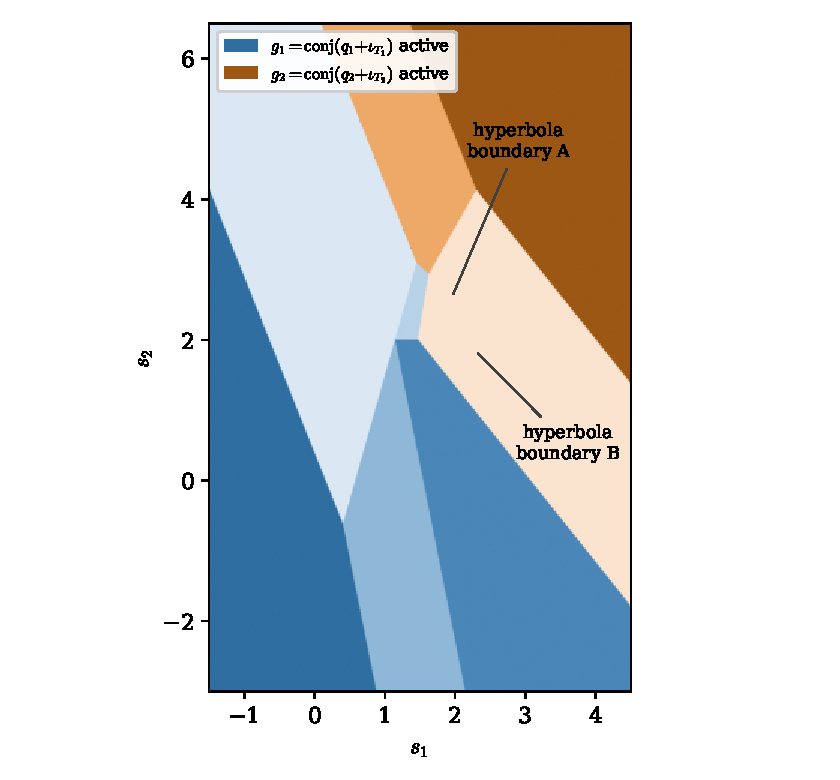
\includegraphics[width=\linewidth]{figures/fig_dual.pdf}\\
  \small $f^*$: the active region of each piece's conjugate, with the
  hyperbolic boundary $A$
\end{minipage}
\caption{The per-piece conjugate of a bilinear two-piece example: the primal
(cells $T_1,T_2$) and the active regions of
$g_k=\operatorname{conj}(q_k+\iota_{T_k})$ whose maximum is $f^*$; the boundary
$A$ on which the maximiser switches is hyperbolic, one of the non-parabolic
edges of Section~3. Source: \texttt{doc/fig\_primal.pdf},
\texttt{doc/fig\_dual.pdf} (design-phase figures of the bilinear-quadrilateral
conjugate discussed in \texttt{ALGORITHM.md}).}
\label{fig:xy}
\end{figure}

\subsection{The cell-interior test, and the star-polygon defect}

The one genuinely hard predicate in the conjugate is: \emph{does this cell have
an interior point} (so that a face is live on it, and so that a row may be
dropped as implied). The repository's test is a witness search -- pairwise
conic/line intersections, then a bounded random probe, then a complete
cylindrical-decomposition sample of the critical abscissae and sector
end-points -- and it has a history worth stating, because it is the one place
the engine was \emph{measurably wrong} on a whole class of inputs.

\paragraph{The defect, found and fixed.}
On \emph{star polygons} -- $2n$ vertices alternating radius $100$ and $45$
around the origin (Figure~\ref{fig:star}), carrying $f=(x^2+y^2)/2$ --
\texttt{conj($f$)} returned values \emph{too low} at some dual points: wrong on
$111/625$ sampled dual points at $n=6$, and wrong on $n=7,8,9,10$ in Rust and
$n=7$ in Python, the engines disagreeing with each other and with the
definition on the class. Two independent causes, both fixed in all three
languages.
% CITE: DECISIONS.md entry 2026-11-17, in full
\begin{enumerate}[label=(\arabic*),leftmargin=*]
\item A line-versus-conic intersection routine multiplied the substituted
  quadratic by $\mathit{scale}^2$ but built the points without the matching
  division, so its roots were $\mathit{scale}\cdot t$ where $t$ was wanted; only
  $|\mathit{scale}|=1$ was right. A missing intersection point is a missing
  witness, so the cell-interior test said ``no interior'' for cells that have
  one, a bounding row was dropped, and the evaluator picked the lower face.
\item When the conics do not meet at all, the fallback probe box was
  $[-4,4]^2$ around the origin, so a cell far from the origin was declared
  empty. The fix adds a \emph{complete} sample search -- a two-dimensional
  cylindrical decomposition of the sign conditions -- as the last resort.
  % CITE: DECISIONS.md 2026-11-17, fix part (2); the code in
  %   \texttt{MATLAB/cellHasInterior.m},
  %   \texttt{python/cca2/cell\_has\_interior.py}, \texttt{rust/src/cells.rs}
\end{enumerate}
After the fix the class verifies against the \emph{definition}, not against
another engine: $n=6,\ldots,16$ in the Rust suite (with $n=17,18,19,20$ as
opt-in long runs of the same test), $n=4,5,6,7$ in the Python suite, the
MATLAB fast suite green, and fold-versus-tree reduction agreeing.
% CITE: rust/tests/star.rs; python/tests/test\_star\_polygons.py; DECISIONS.md
% 2026-11-17 ``Verified''; both test files re-run in this session:
% \texttt{rust/tests/star.rs} (n=6..10 default) not re-run here (no Rust toolchain
% in this environment), the Python star test 4/4 and the kernel and definition
% oracles green, see Section~6.4
 A class-based refusal -- refusing to compute
the conjugate of a strictly convex quadratic on a bounded nonconvex polygon --
was tried and rejected, because it also refuses correct cases (the golden
conjugate record~36, an L-shape).
% CITE: DECISIONS.md 2026-11-17, ``Not
% viable''

\begin{figure}[t]
\centering
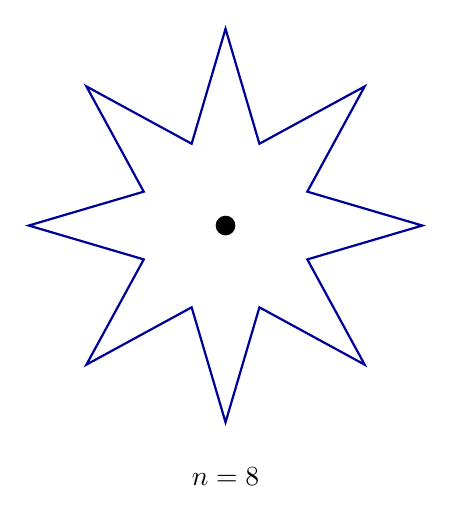
\begin{tikzpicture}[scale=0.025]
  % Star polygon, n = 8 (16 vertices), alternating radii 100 and 45, as in
  % rust/tests/star.rs (the star() constructor) and
  % python/star_defect_diagnosis.py (the same star, same radii).
  \foreach \i in {0,...,15} {
    \pgfmathsetmacro{\ang}{360 * \i / 16}
    \ifodd\i \pgfmathsetmacro{\rr}{45} \else \pgfmathsetmacro{\rr}{100} \fi
    \coordinate (V\i) at ({\rr*cos \ang}, {\rr*sin \ang});
  }
  \draw[thick,blue!60!black] (V0) \foreach \i in {1,...,15} { -- (V\i) } -- cycle;
  \fill (0,0) circle (5);
  \node[below] at (0,-118) {$n=8$};
\end{tikzpicture}
\caption{The star-polygon class of Section~4.2: $2n$ vertices alternating
radius $100$ and $45$, carrying $f=(x^2+y^2)/2$ (here $n=8$). The class on
which \texttt{conj} was wrong (too low) at some dual points before the fix of
Section~4.2; it now verifies against the definition for $n=6,\ldots,16$.
% CITE: rust/tests/star.rs, python/tests/test\_star\_polygons.py, DECISIONS.md
% 2026-11-17
}
\label{fig:star}
\end{figure}

\subsection{What the conjugate returns}

The return value is a \texttt{QuaCon}: a piecewise quadratic function on a
subdivision whose faces are the rational quadratics of
Theorem~\ref{thm:conjface}, whose edges are the rational conics, and whose
vertices are stored as the degree-$\le4$ algebraic points of
Theorem~\ref{thm:deg4} (or, where a vertex is not written down, as the
H-form row of its region -- the repository's discipline of deciding
predicates by resultants and Sturm sequences rather than by coordinates).
% CITE: CONJ\_FIELD\_PROOF.md sections 7--8, ``What this means for the number
% type'' and ``Data structure options''; the type in MATLAB/QuaCon.m
Where a
case is outside the represented family the engine refuses \emph{by name} with a
stable identifier, and the refusal itself is part of the parity contract of
Section~6.
% CITE: the refusal discipline in SUPPORT\_MATRIX.md; rust/README.md
% ``refusals carry the SAME identifier strings''

% ============================================================================
\section{The exact biconjugate and the convex envelope}
% ============================================================================

\subsection{A direct operator, not a composition}

The biconjugate $f^{**}$ is the closed convex envelope. It could be computed as
$\operatorname{conj}(\operatorname{conj}(f))$; the repository does not, because
the composition is a detour -- a second conjugation of an object that is
already convex -- and because the envelope has direct closed forms in the cases
that matter. The dispatch, in order:
\begin{enumerate}[leftmargin=*]
\item normalise (merge same-quadratic adjacent faces, convexity-checked);
\item $f$ convex $\Rightarrow$ return $f$ (nothing to compute; the convexity
  flag is trusted with one free guard -- every piece's Hessian must be positive
  semidefinite, else the flag is refused loudly);
\item $f$ separable on a box $\Rightarrow$ one-dimensional envelopes per axis,
  summed;
\item $f$ bilinear on a box $\Rightarrow$ the McCormick (Al-Khayyal--Falk)
  closed form, in two triangular faces meeting on a diagonal;
  % CITE: ALGORITHM.md, biconj dispatch cases 2--3; the pin
  %   \texttt{biconjugateTest/bilinearOverABoxGivesTheMcCormickEnvelope}
\item $f$ bilinear on a diamond $\Rightarrow$ rotate $45^\circ$, separate,
  rotate back (the one place the rotation pays: it turns the diamond into a box
  and the concave direction into an affine chord);
  % CITE: ALGORITHM.md, case 4, verified against an LP reference at error~$0$
\item a single bounded triangle $\Rightarrow$ the direct Step-1 formula of
  \citet{KARMARKAR-25a}, no conjugation at all;
\item otherwise $\operatorname{conj}(\operatorname{conj}(f))$ -- the exception,
  not the rule.
  % CITE: ALGORITHM.md, biconj dispatch and ``Two invariants worth
  %   exploiting''
\end{enumerate}

\subsection{Atoms, envelope assembly, bridge faces}

The non-convex cases assemble the envelope from \emph{atoms} -- the convex
envelopes of the pieces -- and then take the minimum of their maxima over the
primal subdivision. The pipeline, in the order the repository builds it:
\begin{itemize}[nosep,leftmargin=*]
\item \textbf{atoms}: the convex envelope of each quadratic piece;
  % CITE: the atoms step in biconjAtoms.m; the test biconjAtomsTest.m
\item \textbf{envelope assembly and pruning}: the min-of-maxes of the atoms,
  with faces that are certified \emph{below} another dropped -- the
  empty-set certificate \texttt{algRowFails} decides, in exact arithmetic,
  whether a candidate face's rows can all hold, including the perfect-square
  tangency case \texttt{psTangency}, where a face ties another only on a curve
  and owns no area;
  % CITE: DECISIONS.md entry 2026-11-17 ``the c = -2 diagonal-kink zero-area
  %   faces, dropped: the perfect-square tangency''; the code in
  %   \texttt{MATLAB/algRowFails.m}, \texttt{python/cca2/alg\_row\_fails.py},
  %   \texttt{rust/src/alg\_row\_fails.rs}, pinned by
  %   \texttt{MATLAB/algRowFailsTest.m}, \texttt{MATLAB/algRowFailsSurdTest.m}
  %   and \texttt{rust/tests/ps\_tangency.rs}
\item \textbf{bridge faces}: where two atoms meet along a curve, the envelope
  on the ruled cell between them is one of the algebraic faces of
  Theorem~\ref{thm:biconjface}; the bridge is computed algebraically
  (\texttt{bridgeFaceAlg}) or, in the degenerate single-piece case where the
  incidence conic degenerates to a line, rationally (\texttt{bridgeFaceRat});
  % CITE: the bridge code in MATLAB/bridgeFaceAlg.m,
  %   MATLAB/bridgeFaceRat.m and their tests bridgeFaceAlgTest.m,
  %   bridgeFaceRatTest.m; the degenerate single-piece case in DECISIONS.md
  %   2026-08-23, ``RatPol is the case $H_i=0$ AND $H_j$ rank 1''
\item \textbf{local-arrangement subdivision and min-of-maxes overlay}: the
  subdivision is the local arrangement of the atoms' boundaries, and where
  several atom pairs are active the answer is a min of maxima, returned as
  \texttt{EnvelopeMin} with an overlay budget.
  % CITE: the sequence of decisions in DECISIONS.md 2026-10-18 $\to$
  %   2026-11-05; the overlay budget of $3000$ and the EnvelopeMin default on
  %   Example~2 in TODO.md, lines 100--106, with the whole-overlay measurement of
  %   $3299$ faces in $1247$~s
\end{itemize}

The three output types, and when each occurs:
\begin{center}
\begin{tabular}{p{2.9cm}p{4.6cm}p{7.4cm}}
\toprule
type & when & what it carries \\
\midrule
\texttt{QuaCon} & every atom pair is rational & piecewise quadratic on a
polyhedral subdivision, rational data \\
\texttt{AlgCrv} & an algebraic bridge face is live & the algebraic faces of
Theorem~\ref{thm:biconjface} in the parametrisation of Section~3.2 \\
\texttt{EnvelopeMin} & several atom pairs active, overlay budget reached & the
min-of-maxes directly, with the tuple list \\
\bottomrule
\end{tabular}
\end{center}
\noindent.
% CITE: the type classes in MATLAB/QuaCon.m, MATLAB/AlgCrv.m,
% MATLAB/AlgCon.m; the refusal/type discipline in SUPPORT\_MATRIX.md and
% rust/README.md; the return-type record in RETURN\_TYPE.md
 Refusals outside
this table carry stable identifiers that the Python and Rust ports reproduce,
and which are part of the parity contract of Section~6.

\subsection{Known defects on the envelope side}

Two, stated plainly (the full list with reproduction commands is in the
repository's support matrix).
% CITE: SUPPORT\_MATRIX.md section 7, ``Known
% defects'', and section 7.1
\begin{itemize}[nosep,leftmargin=*]
\item \texttt{getInterior} on a \emph{singular} quadratic: on a piece where $f$
  is constant along an edge the gradient map is not invertible, two edge cells
  come out on the same region, and the first one checked wins. Measured end to
  end: the biconjugate of the parallelogram fixture is about $4\%$ low at $2$
  of $10$ interior probe points ($0.986$ for $1.031$; $1.913$ for $1.950$),
  reproducible in about a minute with
  \texttt{functionNDomainTest.parallelogramPiece9}.
  % CITE: SUPPORT\_MATRIX.md section 7, the LIVE row, and section 7.1
\item the legacy \texttt{'cplq'} engine carries its own open items (the
  $>4$~h poly2 kinks; an \texttt{eig} tolerance that can return $+\infty$ on a
  strictly convex quadratic) -- disclosed in Section~9.2, not a defect of the
  exact engine.
  % CITE: TODO.md ``Open now'', items 4 and 6
\end{itemize}

% ============================================================================
\section{The exact engine and its verification}
% ============================================================================

\subsection{Exact arithmetic, and where doubles appear}

Every exact decision -- face liveness, row-dropping, cell interiors, bridge
witnesses, the emptiness certificate -- is decided in exact arithmetic:
rationals, with integer arithmetic on top of doubles to $2^{53}$ and a
big-integer fallback beyond.
% CITE: the exact kernels in MATLAB/ratQ.m and
% MATLAB/bigZ.m; the Python twin in python/cca2/rat\_q.py with unbounded ints
% and \texttt{fractions.Fraction}; python/bench/RESULTS.md ``What ran''
 In the
ports the FLINT library provides one exact kernel -- the odd-multiplicity part
of a bivariate polynomial's square-free decomposition -- where the pure
implementation is too slow, and everything else stays in the language.
% CITE: python/cca2/\_poly.py header, with the measured hot spot and the
% pure-Python twin as reference; rust/src/flint.rs
 Doubles appear only for
sampling and for the polynomial kernels that have a symbolic oracle; in the
benchmark the Symbolic Math Toolbox is reached only in
\texttt{algRowFails} fallbacks on overflow beyond $2^{53}$, ``not reached here''.
% CITE: python/bench/RESULTS.md ``What ran'' table

\subsection{The four oracles}

The verification harness has four oracles, none of which shares code with the
engine it checks.
% CITE: the design in DECISIONS.md 2026-11-17 and the files
% named below

\begin{enumerate}[label=\textbf{(\arabic*)},leftmargin=*]
\item \textbf{Golden replay.} Every \texttt{conjQ}/\texttt{biconjQ} call the
  MATLAB suites make is recorded as exact-rational JSON lines --
  \texttt{python/golden/*.jsonl}, $9$ files, $2912$ lines: $176$ conjugate
  records, $114$ biconjugate records, the five slow-suite files, and two
  trace files of intermediate calls -- and replayed by the other two engines,
  field for field on \texttt{QuaCon}s, by kind plus sampled values on
  \texttt{AlgCrv}, and by identifier on refusals.
  % CITE: python/golden/ (the files, the line counts); the replay in
  %   python/tests/test\_golden\_\*.py and rust/README.md's verification table:
  %   $176/176$ conjugate, $114/114$ biconjugate, $20/20$ slow-suite records
\item \textbf{Definition oracle.} A MATLAB-free check that computes the
  conjugate \emph{pointwise} from the definition
  $f^*(s)=\sup_x(\langle s,x\rangle-f(x))$ using KKT candidates, sharing
  nothing with \texttt{conjQ}; and that the biconjugate is a convex minorant
  of $f$ equal to $\langle s,x\rangle-f^*(s)$ at its own gradient.
  % CITE: python/cca2/check.py and python/tests/test\_definition.py, which run
  %   the oracle on every non-refusal golden fixture; $186$ fixtures, green in
  %   this session (Section~6.4)
\item \textbf{Kernel oracle.} The exact polynomial kernels are checked against
  a symbolic (SymPy) oracle, with a lint test that keeps SymPy out of the
  production path.
  % CITE: python/tests/test\_kernel\_oracle.py and test\_no\_cas.py; $187$
  %   tests, green in this session (Section~6.4)
\item \textbf{Cross-engine parity.} MATLAB, Python and Rust agree field for
  field on the goldens, and the Rust engine's digest of the \emph{complete}
  result (every face, row and coefficient, in order) of all $200$ benchmark
  fixtures is identical at $1$, $2$, $8$ and $32$ threads to the digest taken
  from the serial engine before any parallelism was added.
  % CITE: rust/tests/parallel.rs (the digest test, against
  %   \texttt{bench/parallel/digest\_serial.tsv}); rust/README.md verification
  %   table; the re-baselining after the star fix in DECISIONS.md 2026-11-17
\end{enumerate}

\paragraph{Why the harness is a contribution.}
The star-polygon defect of Section~4.2 was \emph{visible} only because oracle
(4) compared the three engines and oracle (2) compared all of them against the
definition: the engines disagreed with each other and with the definition on
the same class, which localised the fault to a shared routine rather than to a
port.
% CITE: DECISIONS.md 2026-11-17; python/star\_defect\_diagnosis.py, which
% now reports the defect as NOT reproduced
 Without the harness, a wrong value
on one input class of a nonconvex function is invisible to every test that
passes.

\subsection{Test statistics}

The committed state of the suites, with the files that carry the measurements:

\begin{center}
\begin{tabular}{p{2.8cm}p{5.7cm}p{6.3cm}}
\toprule
engine & result & supporting record \\
\midrule
MATLAB (reference) & fast bucket $834/0$; normal bucket $35/0$; the eight
  exact slow suites green (kink $3/0$, min-subdivision $4/0$, erratum
  Example~2 $4/0$, algCrv $3/0$, envelope-slow $1/0$, algRowFails-surd $5/0$,
  unbounded-face $19/0$, guard-symbolic $11/0$) & \texttt{DECISIONS.md}
  entries 2026-11-17 (fast, post-star-fix) and 2026-11-11 (normal and slow);
  measured on the shared machine (Frances)
  % CITE: DECISIONS.md, those entries
\\
Python & $2741$ tests pass & \texttt{DECISIONS.md} 2026-11-17;
  % CITE: DECISIONS.md 2026-11-17, ``Verified''
  the per-oracle files of
  Section~6.2
  % CITE: python/tests/
\\
Rust & full test pass (goldens replayed against the Python reference, with and
  without FLINT; digest parity at $1/2/8/32$ threads; the star suite
  $n=6,\ldots,10$ plus opt-in $n=11,\ldots,20$) & \texttt{DECISIONS.md}
  2026-11-17, ``Verified''; \texttt{rust/README.md}
  % CITE: rust/README.md verification table; rust/tests/parallel.rs;
  %   rust/tests/star.rs
\\
\bottomrule
\end{tabular}
\end{center}

\noindent
The per-stage cache that makes the MATLAB slow suites splittable is
\texttt{plqStage.m}; the definition verifiers of the MATLAB suites are
\texttt{plqCheck.m} ($\co f \le f$ with equality at vertices; $f^*(s)$ against
a numeric sup; $f^{**}\le f$ and convex on sampled segments).
% CITE: CLAUDE.md ``Tools that already exist''

\subsection{What was re-run in this session}

MATLAB cannot run in this environment (the licence server is on campus, behind
the VPN), so the MATLAB rows of the table above stand at their committed
measurements; the Python rows were re-run here, all green:
\begin{center}
\begin{tabular}{p{4.8cm}p{2.8cm}p{7.4cm}}
\toprule
suite & result (this session, 2026-11-19) & command \\
\midrule
kernel oracle (SymPy) & $187$ passed &
 \texttt{python3 -m pytest tests/test\_kernel\_oracle.py -q} \\
 star polygons $n=4,5,6,7$ (definition oracle) & $4$ passed &
 \texttt{python3 -m pytest tests/test\_star\_polygons.py -q} \\
 definition oracle, all $186$ fixtures & $186$ passed &
 \texttt{python3 -m pytest tests/test\_definition.py -q} \\
\bottomrule
\end{tabular}
\end{center}

\subsection{Case study: three MATLAB defects the port found}

The harness's value is not theoretical: during the port, three places where the
MATLAB reference and the Python twin disagreed were \emph{MATLAB's fault}, each
found by a replay, each with a red-first test, and each a silent wrong answer
or a silent wrong count:
% CITE: DECISIONS.md entry 2026-11-11, in full
\begin{enumerate}[label=(\arabic*),leftmargin=*]
\item \texttt{ratQ.sturmChain} lost the Sturm property when a chain element
  had a negative leading coefficient and the degree dropped by~$2$: a wrong
  root \emph{count}, silent. Measured: \texttt{ratQ.countRootsIn} returned $0$
  for a quartic with two real roots in the interval.
\item \texttt{cellSamplePoint} accepted a sample lying \emph{on} a boundary
  line, so a cell of \emph{zero width} was live and the subdivider emitted
  bridge faces for it (faces that own no point).
\item \texttt{linealityConj} conjugated the numerator of a rational face
  instead of the fraction: a wrong \emph{value}, silent -- $f=x^2/3$ on
  $x\ge0$ gave $f^*(2,0)=1$ where the supremum is $3$.
\end{enumerate}
The fixes are pinned by tests that fail against the pre-fix code.
% CITE: DECISIONS.md 2026-11-11, the test names in each item; the red-first
% discipline in the same entry

% ============================================================================
\section{Implementations and performance}
% ============================================================================

\subsection{Three engines, one corpus}

The engine exists in three languages, each a module-for-module port of the
previous, all at parity on the recorded corpus:
\begin{itemize}[nosep,leftmargin=*]
\item \textbf{MATLAB} (the reference, \texttt{MATLAB/}): base MATLAB R2024a,
  no toolbox required for the compute path; exact integers are
  double-precision to $2^{53}$ then \texttt{java.math.BigInteger}.
  % CITE: python/bench/RESULTS.md ``What ran''; the Symbolic Math Toolbox is
  %   touched only in \texttt{algRowFails} fallbacks on overflow and by the legacy
  %   \texttt{'cplq'} suites, which are presented as a cross-check, not as the
  %   result
\item \textbf{Python} (\texttt{python/cca2/}): a module-for-module port,
  unbounded integers and \texttt{fractions.Fraction} for the exact layer,
  with optional accelerators -- \texttt{python-flint} for one square-free
  kernel and \texttt{numba} for the Bernstein sign tests -- each switchable off
  with identical answers \cite{FLINT-26,NUMBA-20}.
  % CITE: python/PORT\_NOTES.md, python/PORT\_PLAN.md; the accelerator record
  %   and its measured effect in python/bench/RESULTS.md addenda;
\item \textbf{Rust} (\texttt{rust/}): a port of the Python port,
  \texttt{num-bigint}/\texttt{num-rational} for the exact layer, FLINT
  optional for the same one kernel, and a \texttt{rayon} parallelisation of
  the per-cell and per-tuple loops with the reduction left by default \cite{FLINT-26,RAYON-21}.
  % CITE: rust/README.md; rust/PARALLEL.md;
\end{itemize}

Parity is not asserted, it is tested: the golden replay of Section~6.2
(field-for-field on \texttt{QuaCon}s, by identifier on refusals, $176/176$ and
$114/114$), the slow-suite replay ($20/20$, including the $317$-face kink
\texttt{AlgCrv} and the Example-2 \texttt{EnvelopeMin}), with and without
FLINT,
% CITE: rust/README.md verification table
and the digest parity of the
$200$ fixtures across thread counts.
% CITE: rust/tests/parallel.rs

\subsection{The 200-fixture protocol}

The benchmark corpus is the $200$ distinct exact inputs the MATLAB suites pass
to \texttt{conjQ}/\texttt{biconjQ}, derived from the goldens into plain JSON
(\texttt{python/bench/fixtures.json}); it is the data component of the
artifact -- a referee can replay the benchmark with neither MATLAB nor any of
the paper's engines, from the JSON alone.
% CITE: python/bench/fixtures.json
% (the $200$ entries, verified in this session); python/bench/make\_fixtures.py
The protocol
% CITE: python/bench/bench\_matlab.m, bench\_python.py,
% compare.py; rust/bench/ (the same protocol in Rust)
: each fixture is timed
first call plus three repetitions (or once, if the first call took over $20$~s),
best per fixture, two passes, and the engine's own per-call memos are emptied
before every timed call so that repetitions are not flattered by warm caches.

\subsection{Results}

The committed numbers, with their sources and caveats:

\begin{table}[t]
\centering
\begin{tabular}{p{4.2cm}p{3.1cm}p{1.9cm}p{5.7cm}}
\toprule
engine & all $200$ fixtures (s) & vs MATLAB & source \\
\midrule
MATLAB R2024a (reference) & $1126$ & $1\times$ &
 \texttt{python/bench/RESULTS.md} (run5, ``After the EnvelopeMin speed-up'') \\
 Python (\texttt{numba} + \texttt{FLINT}) & $88.5$ & $12.7\times$ &
 \texttt{python/bench/RESULTS.md} (same section) \\
 Rust, 1 thread (\texttt{FLINT}) & $15.7$ & $72\times$ &
 \texttt{rust/bench/RESULTS.md} (all row) \\
 Rust, 32 threads & $2.22$ & $\approx 500\times$ &
 \texttt{rust/PARALLEL.md} (final sweep, 32-thread row) \\
\bottomrule
\end{tabular}
\caption{The $200$-fixture corpus, best times per fixture summed
(Section~7.3). All four columns are committed runs on the shared machine
(Frances), on different days and under different loads; read the ratios as
indicative, not as a ranking (Section~7.4).}
\label{tab:speed}
\end{table}

The heaviest fixtures, single thread to $32$ threads:
% CITE: rust/bench/RESULTS.md slowest-fixture table; rust/PARALLEL.md final sweep
the kink biconjugate ($317$-face \texttt{AlgCrv}) goes from $7.56$~s to
$0.81$~s; erratum Example~2 (\texttt{EnvelopeMin}) from $5.36$~s to $0.73$~s;
the min-subdivision biconjugate from $1.44$~s to $0.29$~s.

\subsection{Caveats, stated with the numbers}

These timings come from a shared machine (Frances, $64$ cores), on different
days, under load averages between $0.3$ and $16$, with up to four benchmark
processes concurrent; the repository's own caution -- ``read the ratios as
indicative, not exact'' -- carries into this paper, and the numbers are quoted
as the state of the committed runs, not as a ranking of the languages.
% CITE: python/bench/RESULTS.md ``Read with care''; rust/bench/RESULTS.md
% header; rust/PARALLEL.md sweep headers, which record the load during each
% sweep
 In particular: the Python column of Table~\ref{tab:speed} was measured
on \texttt{2026-11-11} with \texttt{numba} and \texttt{python-flint} enabled
and is the last committed run of that configuration; the Rust single-thread
column is from \texttt{2026-11-13}; the $32$-thread column from the
\texttt{2026-11-13}/\texttt{2026-11-15} sweeps recorded in \texttt{PARALLEL.md}.
% CITE: the dates in the headers of those files
 A controlled re-run
(min-of-repetitions, load recorded, quiet machine) is the outstanding step
before these numbers are citable as a performance claim, and is recorded as
such in the repository's gap list.
% CITE: manuscript/outline.md gap G6; the umbrella timing rule in
% \texttt{../CLAUDE.md} section 3

% TODO(G3): no comparison against an independent external implementation or
% against grid/LP-based envelopes exists in the repository yet (outline gap
% G3). The legacy 'cplq' engine is a same-problem comparison only, and it is
% not benchmarked against the exact engine on accuracy or speed. Do not add a
% comparison table to this section before that work is committed.

\subsection{Reproducibility}

The benchmark is reproducible from the repository alone: the fixtures are
plain JSON, the scripts are committed (\texttt{python/bench/},
\texttt{rust/bench/}), and the digest of every fixture's complete result is
recorded (\texttt{rust/bench/parallel/digest\_serial.tsv}), so a re-run is
checked against the committed answers, not against a wall-clock number.
% CITE: rust/tests/parallel.rs (the digest is the assertion);
% rust/bench/parallel/digest\_serial.tsv; the re-baselining after the star fix
% and the psTangency fix, with the old baselines kept, in DECISIONS.md
% 2026-11-17

% ============================================================================
\section{Case studies}
% ============================================================================

\subsection{The counterexample, end to end}

The three-piece example of Theorem~\ref{thm:counter} is the paper's worked
example, because it is at once the simplest refutation of the published
parabolic-subdivision claim and a fully computed instance of the exact engine's
output: the input is a continuous PLQ on one triangle with three
positive-deficient rational pieces; the conjugate carries the elliptic edge
$93s_1^2+38s_1s_2-6s_1+39s_2^2-482s_2-1003=0$; and the switching point
$s^*=\bigl(\frac{-17}{62}+\frac{\sqrt{612\,030}}{186},\frac32\bigr)$ is
algebraic of degree~$2$, with the value $2.9278190688\ldots$ confirmed to five
digits by an independent eight-million-point grid sup.
% CITE: doc/QuaConExample.md, sections 1--2, all numbers there
 The five-piece
version is the harder instance -- it is the one that carries the $S_4$ vertex
of Example~\ref{ex:s4} -- and its conjugate is displayed in full in the
repository: $17$ faces, $41$ edges of which none is a genuine parabola, with
the face table and the edge-by-edge classification.
% CITE: doc/QuaConExample.md section 3; Figure~\ref{fig:facemap}

\subsection{The heavy biconjugates}

Two fixtures carry the algebraic machinery of Section~5 to its limits, and
both are in the benchmark corpus.
% CITE: python/bench/fixtures.json entries
% $191$ and $196$, sourced from \texttt{slow\_erratumBiconjEx2Test} and
% \texttt{slow\_kinkSubdivisionTest}

\paragraph{The kink fixture.}
A continuous PLQ whose biconjugate is a $317$-face \texttt{AlgCrv}: the
algebraic bridge faces of Theorem~\ref{thm:biconjface} are live, and the
subdivision is the local arrangement of Section~5.2. It is the heaviest
conjugate-side fixture in the corpus: $412$--$427$~s in MATLAB, $41$--$45$~s
in Python with the accelerators, $7.56$~s in Rust single-thread, $0.81$~s at
$32$ threads.
% CITE: python/bench/RESULTS.md slowest-fixture tables (the last
% two sections); rust/bench/RESULTS.md; rust/PARALLEL.md final sweep; the face
% count in rust/README.md verification table and DECISIONS.md 2026-11-03
% sequence

\paragraph{Erratum Example~2.}
A biconjugate for which several atom pairs are active and the overlay budget
($3000$ faces) is reached, so the engine returns the \texttt{EnvelopeMin}
directly rather than a subdivided face set; the full overlay was measured at
$3299$ faces in $1247$~s on the MATLAB reference. It is $566$~s in MATLAB,
$27$~s in Python, $5.36$~s in Rust single-thread, $0.73$~s at $32$ threads.
% CITE: TODO.md lines 100--106 (the budget and the overlay measurement);
% DECISIONS.md 2026-11-04 (budget $4000\to3000$); python/bench/RESULTS.md and
% rust/bench/RESULTS.md slowest-fixture tables; rust/PARALLEL.md final sweep

\subsection{The star-polygon class}

After the fix of Section~4.2, the star polygons of Figure~\ref{fig:star} are
the paper's standing test that the cell-interior predicate is complete enough
on nonconvex bounded inputs: the conjugate now verifies against the definition
for $n=6,\ldots,16$ (Rust, with $n=17,\ldots,20$ as opt-in long runs) and
$n=4,\ldots,7$ (Python), with the engines agreeing.
% CITE: rust/tests/star.rs; python/tests/test\_star\_polygons.py; DECISIONS.md
% 2026-11-17 ``Verified'' and ``Not run''; TODO.md, the recorded note that
% $n=17$ is a $>30$-minute run
 We state the range honestly: the class is
verified \emph{up to} $n=16$; beyond that the runs have not been completed and
the claim does not extend.

\subsection{Declared limitations}

Collected here, with their reproduction or source, so that the paper's claims
and its gaps sit in one place:
% CITE: SUPPORT\_MATRIX.md section 7; TODO.md
% ``Open now''; manuscript/outline.md gaps G1--G8
\begin{itemize}[nosep,leftmargin=*]
\item \textbf{One small wrong-value class on the envelope side.}
  \texttt{getInterior} on a singular quadratic leaves two edge cells on the
  same region; measured end to end the parallelogram fixture's biconjugate is
  about $4\%$ low at $2$ of $10$ interior probe points, reproducible in about a
  minute with \texttt{functionNDomainTest.parallelogramPiece9}.
  % CITE: SUPPORT\_MATRIX.md section 7, the LIVE row, and section 7.1
\item \textbf{The star class beyond $n=16$.} Not yet run (multi-hour runs);
  the fix is verified up to $n=16$.
  % CITE: TODO.md, the $n=17$ note
\item \textbf{No independent external comparison.} The correctness claims rest
  on the in-repository oracles of Section~6, which share the repository's own
  definitions; the planned geometric oracle (a CGAL-based cross-check
  generator, deliberately outside this repository) does not exist as a project
  yet, and the external ground-truth registry intended to serve that role has
  no DOI yet
  % TODO(G3): close by adding the external comparison and the DOI'd
  % ground-truth set, then state it in Section 7 instead of this disclaimer.
  % CITE: manuscript/outline.md gaps G3 and G8; the convexdb sequencing in the
  %   cross-project plan referenced by manuscript/outline.md section 5
\item \textbf{No citable release.} The software is alpha with no tagged
  release and no code DOI; the API is still changing (the \texttt{RatPol}
  operators \texttt{conj}/\texttt{biconj}/\texttt{add} and \texttt{partialConj}
  are unimplemented)
  % TODO(G5): close by cutting the tagged release and minting the code DOI,
  % then replace this item with the archive and its DOI in Section 9.
  % CITE: README.md ``Status'' and operators table; SUPPORT\_MATRIX.md
  %   sections 2 and 8
\item \textbf{The legacy engine's open items.} The \texttt{'cplq'} symbolic
  engine, the implementation of \citet{KARMARKAR-25,KARMARKAR-25a}, carries
  its own open items -- the $>4$~h poly2 kinks and an \texttt{eig} tolerance
  that can return $+\infty$ on a strictly convex quadratic -- which are its,
  not the exact engine's, and are disclosed rather than fixed here.
  % CITE: TODO.md ``Open now'', items 4 and 6
\end{itemize}

% ============================================================================
\section{Code and data availability}
% ============================================================================

\subsection{What a referee needs}

Stated plainly:
% CITE: the allocation in manuscript/outline.md section 5,
% itself from the venue record in TODO.md 2026-09-03 and the cross-project plan
% it references
\begin{itemize}[nosep,leftmargin=*]
\item \textbf{To run the reference implementation and the MATLAB suites:}
  MATLAB, academic licence, \emph{no toolbox required for the compute path}.
  The exact engine (\texttt{conjQ}, \texttt{biconjQ}) and the whole
  fast/normal bucket run on base MATLAB R2024a; exact integers are
  double-precision to $2^{53}$ then \texttt{java.math.BigInteger}. The Symbolic
  Math Toolbox is touched only in \texttt{algRowFails} fallbacks on overflow
  (not reached in the benchmark) and by the legacy \texttt{'cplq'} suites,
  which are a cross-check, not the result.
  % CITE: python/bench/RESULTS.md ``What ran''; the MATLAB-suite split in
  %   .claude/suite.sh (fast/normal/slow/verylong buckets, one process per slow
  %   suite because symbolic calls are not interruptible from M-code)
 The
  authors' own machines additionally route the licence server through a campus
  VPN -- an author-side constraint, not a referee-side one, and the reason the
  MATLAB-free routes below are first-class.
\item \textbf{To run without MATLAB at all:} Python~3 or Rust. The Python port
  is complete for \texttt{conjQ}/\texttt{biconjQ} and its test suite is
  MATLAB-free (golden replay from the JSON data, the KKT definition oracle,
  the symbolic kernel oracle, and the rest of the suite); the Rust port
  replays the same goldens against the Python reference and carries the
  $200$-fixture digest tests; FLINT is optional in both, with a slower pure
  implementation giving identical answers.
  % CITE: python/README.md, python/tests/; rust/README.md (the FLINT
  %   optional, and the switches \texttt{CCA2\_FLINT}/\texttt{CCA2\_FLINT\_BUILD})
\item \textbf{The data files.} The test corpus is \emph{plain JSON data, not
  MATLAB code}: \texttt{python/golden/*.jsonl} ($9$ files, $2912$ lines, exact
  rational coefficients) and \texttt{python/bench/fixtures.json} (the $200$
  distinct exact inputs). They are the artifact's data component: a referee can
  verify parity and replay the benchmark with neither MATLAB nor the paper's
  engines.
  % CITE: python/golden/ (verified in this session: $9$ files, $2912$ lines);
  %   python/bench/fixtures.json ($200$ entries, verified in this session)
\end{itemize}

\subsection{Compliance, item by item}

The venue requires code-and-data submission with independent verification of
computational results, and its verification assumes a referee can run the code;
the free route is the journal's green self-archiving, with no APC.
% CITE: manuscript/outline.md section 5, from TODO.md 2026-09-03 and the
% cross-project plan it references

\begin{center}
\begin{tabular}{p{4.9cm}p{7.0cm}p{2.5cm}}
\toprule
requirement & how this work meets it & state \\
\midrule
code available, runnable by a referee & three implementations, two of them
MATLAB-free; base MATLAB for the third; the MATLAB dependency to be declared
in the cover letter & met \\
data available & the exact-rational JSON corpus plus the $200$-fixture bench
protocol, plain text in the archive & met \\
independent verification of results & four oracles sharing no code with the
engine; three engines agreeing at parity; refusal identifiers stable across
engines & met \\
reproducible computational results & benchmark protocol and scripts committed
(\texttt{python/bench/}, \texttt{rust/bench/}); digests recorded as the
assertion; timings caveated (shared machine) & met, caveated \\
citable artifact & -- & \textbf{gap: TODO(G5)}
% TODO(G5): no release tag, no code DOI yet; the convexdb citation the work
% carries also needs its DOI (G3). Close before submission.
\\
\bottomrule
\end{tabular}
\end{center}

\subsection{Declared limitations (cross-reference)}

The limitations of Section~8.4 -- the singular-quadratic envelope defect, the
star class beyond $n=16$, the absence of an independent external comparison,
the absence of a citable release, the legacy engine's open items, and the
shared-machine caveat on all timings -- are the paper's declared limitations,
and they are carried into the cover letter as such rather than discovered by a
referee.

% ============================================================================
\section{Conclusion and open problems}
% ============================================================================

The conjugate and the convex envelope of a bivariate PLQ function are, on
rational data, exact objects of a finite and now-characterised type: rational
faces and edges on the conjugate side, algebraic vertices of degree at most~$4$
with $S_4$ attained, algebraic faces of degree at most~$4$ on the envelope side.
The paper gives direct exact-arithmetic algorithms for both operators, a
verification harness of four code-independent oracles against which every claim
is pinned by a committed test, and three implementations at parity with a
reproducible benchmark. The open problems, in the order the repository keeps
them:
\begin{enumerate}[label=(\roman*),leftmargin=*]
\item the \textbf{singular-quadratic envelope defect} of Section~8.4, a small
  wrong-value class in the same operator as the main claims;
  % CITE: SUPPORT\_MATRIX.md section 7
\item the \textbf{star class beyond $n=16$}, the long runs that would close the
  range;
  % CITE: TODO.md, the $n=17$ note
\item the \textbf{missing operators} of the public API
  (\texttt{RatPol.conj}/\texttt{biconj}/\texttt{add}, \texttt{partialConj}),
  which the exact engine is the substrate for;
  % CITE: README.md operators
  %   table; SUPPORT\_MATRIX.md sections 2 and 8
\item the \textbf{consumer} of the whole enterprise: the SCIP/QPLIB
  integration, whose readiness plan is measured and whose gate conditions
  (bugs ironed out, direct-formula scope clear, timing understood) are stated
  in the repository;
  % CITE: SCIP\_READINESS.md; SUPPORT\_MATRIX.md sections
  %   0.0 and 0.0.1
\item the \textbf{external oracle set} and the \textbf{citable artifact}, the
  two gaps G3 and G5 of Section~8.4, which block a submission but not the
  mathematics
  % TODO(G3) TODO(G5): close before submission; see the TODO comments in
  % Sections 7.4 and 9.2.
  % CITE: manuscript/outline.md gaps G3, G5
\end{enumerate}

\bibliographystyle{plainnat}
\bibliography{biblio}

\end{document}
